% !TeX root = ../../../main.tex
% Nội dung Transaction đã chốt; có thể chỉnh sửa trực tiếp trong file này.
\txsection{Đánh giá hiệu năng và lựa chọn DBMS}\label{sec:tx-3}
Phần này so sánh hiệu năng transaction của \textbf{Oracle và Redis ở cấp cơ sở dữ liệu}, đồng thời đánh giá thời gian xử lý một luồng nghiệp vụ ShopFlash trên \textbf{backend sử dụng Oracle}. Hai phép đo được phân tích riêng vì không có cùng đơn vị công việc.

\txsubsection{Thiết kế benchmark và các chỉ số đánh giá}\label{sec:tx-3-1}
Benchmark được thực hiện ngày \textbf{27/10/2026} trên máy Ryzen AI 7 PRO 350 (8 nhân/16 luồng), RAM 26 GiB, sử dụng Oracle Database Free, Redis 7.4.7, Java 21 và k6 0.55.2. Các kết quả phản ánh môi trường local, chưa được cô lập tài nguyên như production.

\begin{table}[!htbp]
\centering
\caption{Các tham số cấu hình workload của benchmark.}\label{tab:tx-17}
\reporttablesetup
\begin{tabularx}{\linewidth}{|>{\hsize=0.9\hsize\linewidth=\hsize}L|>{\hsize=0.45\hsize\linewidth=\hsize}L|>{\hsize=1.65\hsize\linewidth=\hsize}L|}
\hline
\rowcolor{ReportTableHead}
\reportheader{Tham số} & \reportheader{Giá trị} & \reportheader{Ý nghĩa} \\ \hline
\texttt{cart\_\allowbreak{}size} & 1, 5 & Số dòng sản phẩm trong một Checkout \\ \hline
\texttt{concurrency} & 1, 10 & Số worker hoặc người dùng ảo thực thi đồng thời \\ \hline
\texttt{warmup} & 50 & Số lượt làm nóng, không tính vào kết quả \\ \hline
\texttt{rounds} & 5 & Số lượt đo cho mỗi tổ hợp \\ \hline
\texttt{samples\_\allowbreak{}per\_\allowbreak{}round} & 200 & Tổng số transaction hoặc flow trong một lượt \\ \hline
\texttt{fixture\_\allowbreak{}stock} & 100 & Tồn kho khởi tạo trong database benchmark \\ \hline
\texttt{quantity\_\allowbreak{}per\_\allowbreak{}line} & 1 & Số lượng mua của mỗi dòng sản phẩm \\ \hline
\end{tabularx}
\end{table}
Mỗi tổ hợp có \textbf{5 \(\times\) 200 = 1.000 mẫu chính thức}. Mức \texttt{concurrency =\allowbreak{} 10} nghĩa là mười worker/VU cùng xử lý tổng cộng 200 mẫu mỗi round, không phải mỗi worker xử lý 200 mẫu. Theo đó, phép đo cấp cơ sở dữ liệu có \textbf{8.000 transaction} (2 DBMS \(\times\) 2 Cart Size \(\times\) 2 Concurrency \(\times\) 1.000); phép đo HTTP trên Oracle có \textbf{4.000 flow} (2 Cart Size \(\times\) 2 Concurrency \(\times\) 1.000).

Các chỉ số chính gồm \textbf{p50/p95 latency} (ms) — thời gian mà lần lượt 50\%/95\% mẫu thành công hoàn tất không chậm hơn; \textbf{TPS} — số transaction thành công mỗi giây; và \textbf{Flow/s} — số luồng nghiệp vụ hoàn thành mỗi giây. Benchmark đồng thời ghi nhận lỗi, yêu cầu bị từ chối và \textbf{invariant violations} để kiểm tra tính đúng đắn. Các phân vị trong bảng được tính trên các mẫu thành công; độ dao động giữa năm round được thể hiện qua trung bình và độ lệch chuẩn (SD).

\txsubsection{Kết quả Database-level Benchmark}\label{sec:tx-3-2}
Benchmark thực thi Checkout mô phỏng \textbf{trực tiếp qua JDBC/Jedis}, không qua HTTP. Oracle sử dụng bảng quan hệ và transaction; Redis sử dụng các \textbf{String key} với \texttt{WATCH/\allowbreak{}MULTI/\allowbreak{}EXEC}, không phải Lua/Hash của Mục~\ref{sec:tx-2}.

\begin{table}[!htbp]
\centering
\caption{Khác biệt giữa hai implementation trong database benchmark.}\label{tab:tx-18}
\reporttablesetup
\begin{tabularx}{\linewidth}{|>{\hsize=0.7\hsize\linewidth=\hsize}L|>{\hsize=1.15\hsize\linewidth=\hsize}L|>{\hsize=1.15\hsize\linewidth=\hsize}L|}
\hline
\rowcolor{ReportTableHead}
\reportheader{Đặc điểm} & \reportheader{Oracle} & \reportheader{Redis} \\ \hline
Dữ liệu & Các bảng Cart, Order, Order Item và Inventory & String key mô phỏng Cart, Order, Price và Stock \\ \hline
Kiểm soát transaction & Constraint, row lock, \texttt{COMMIT} & Java validation, \texttt{WATCH/\allowbreak{}MULTI/\allowbreak{}EXEC} \\ \hline
Kết nối & JDBC connection pool & Jedis connection riêng cho mỗi worker \\ \hline
Hậu kiểm & Order/Order Items, Inventory và Cart & Các key Order, Stock và Cart \\ \hline
\end{tabularx}
\end{table}
Hai implementation có cùng mục tiêu Checkout nhưng khác cấu trúc dữ liệu và chi phí xử lý. Đáng chú ý, thời gian đo Oracle bao gồm bước lấy connection từ pool, còn Jedis connection đã được chuẩn bị trước, nên kết quả chỉ phản ánh \textbf{hai cách triển khai trong điều kiện khảo sát}, không phải so sánh hai engine với chi phí hoàn toàn tương đương.

\begin{table}[!htbp]
\centering
\caption{Kết quả Database-level Benchmark. p50/p95 tính trên 1.000 mẫu thành công của mỗi tổ hợp; TPS dựa trên tổng thời gian thực của năm round. Nguồn: \texttt{results/\allowbreak{}summary-\allowbreak{}20261027/\allowbreak{}database-\allowbreak{}summary.\allowbreak{}csv}.}\label{tab:tx-19}
\reporttablesetup
\scriptsize
\begin{tabularx}{\linewidth}{|>{\hsize=0.8\hsize\linewidth=\hsize}L|>{\hsize=1.05\hsize\linewidth=\hsize}L|>{\hsize=0.85\hsize\linewidth=\hsize}L|>{\hsize=1.1\hsize\linewidth=\hsize}L|>{\hsize=1.1\hsize\linewidth=\hsize}L|>{\hsize=1.1\hsize\linewidth=\hsize}L|}
\hline
\rowcolor{ReportTableHead}
\reportheader{Cart Size} & \reportheader{Concurrency} & \reportheader{DBMS} & \reportheader{p50 (ms)} & \reportheader{p95 (ms)} & \reportheader{TPS} \\ \hline
1 & 1 & Oracle & 0,8712 & 1,3416 & 847,36 \\ \hline
1 & 1 & Redis & 0,1303 & 0,2109 & 4.517,08 \\ \hline
1 & 10 & Oracle & 2,2116 & 3,0110 & 3.503,15 \\ \hline
1 & 10 & Redis & 0,5125 & 0,6970 & 12.288,94 \\ \hline
5 & 1 & Oracle & 2,0081 & 2,6394 & 404,74 \\ \hline
5 & 1 & Redis & 0,2995 & 0,4590 & 1.787,83 \\ \hline
5 & 10 & Oracle & 4,5749 & 6,1164 & 1.753,74 \\ \hline
5 & 10 & Redis & 0,9906 & 1,4019 & 5.438,86 \\ \hline
\end{tabularx}
\end{table}
\begin{figure}[!htbp]
\centering
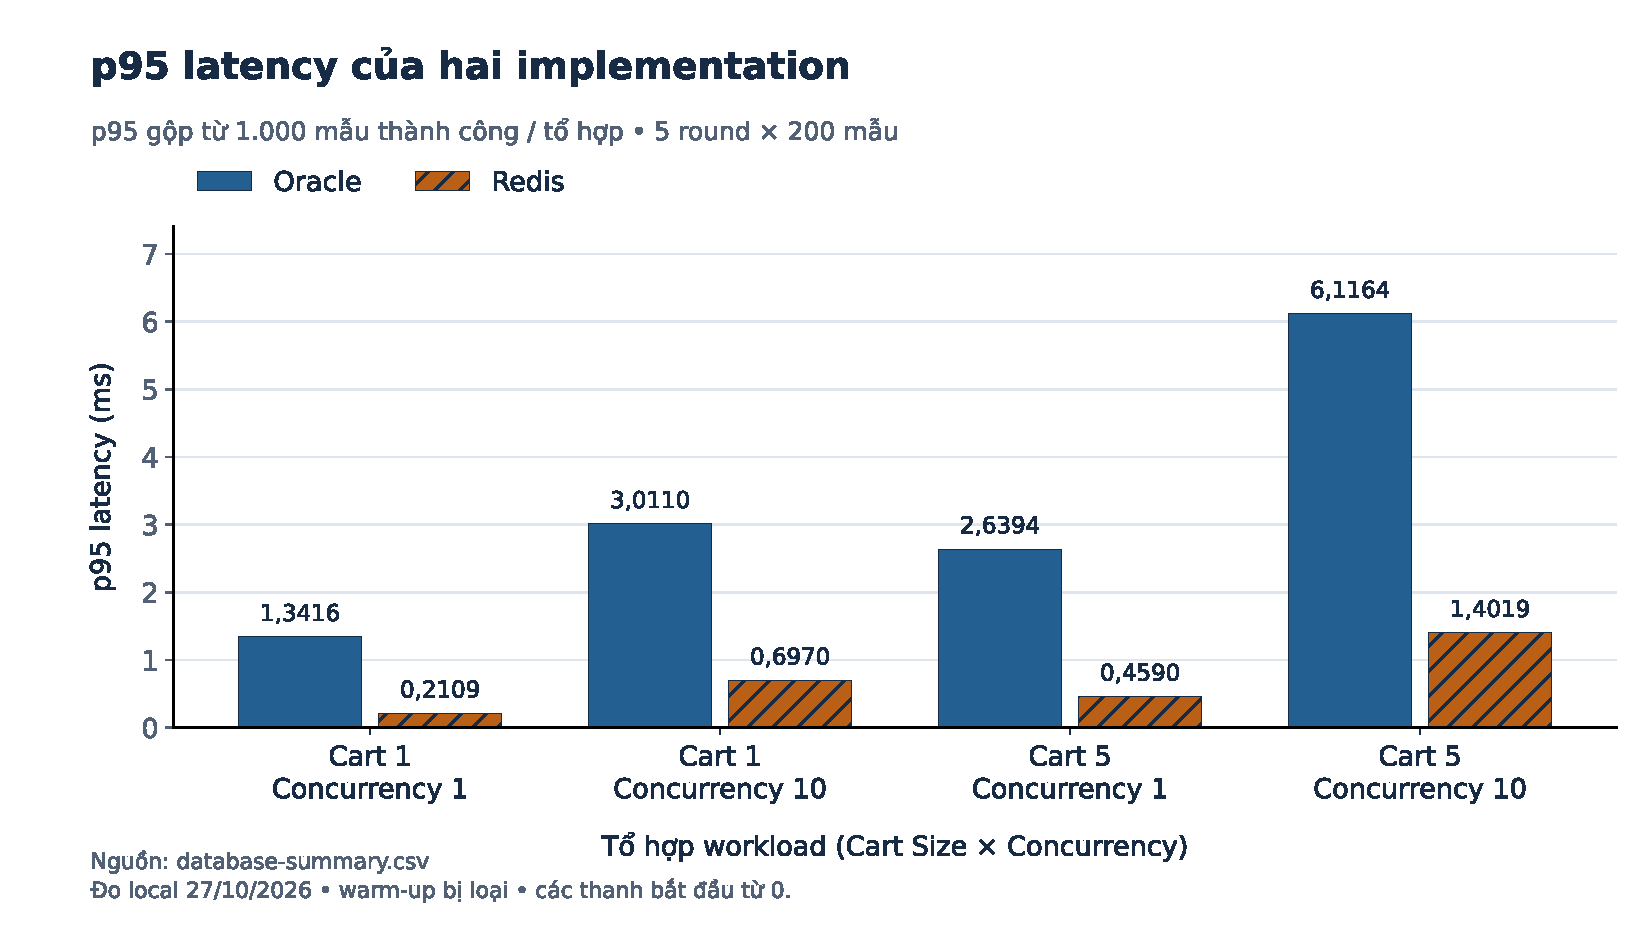
\includegraphics[width=\linewidth]{Pictures/Task_4/4.3-01-database-p95.pdf}
\caption[So sánh p95 latency Oracle–Redis theo Cart Size và Concurrency]{So sánh p95 latency Oracle–Redis theo Cart Size và Concurrency; dữ liệu từ bảng Database-level Benchmark, đơn vị ms.}\label{fig:tx-1}
\end{figure}
\begin{figure}[!htbp]
\centering
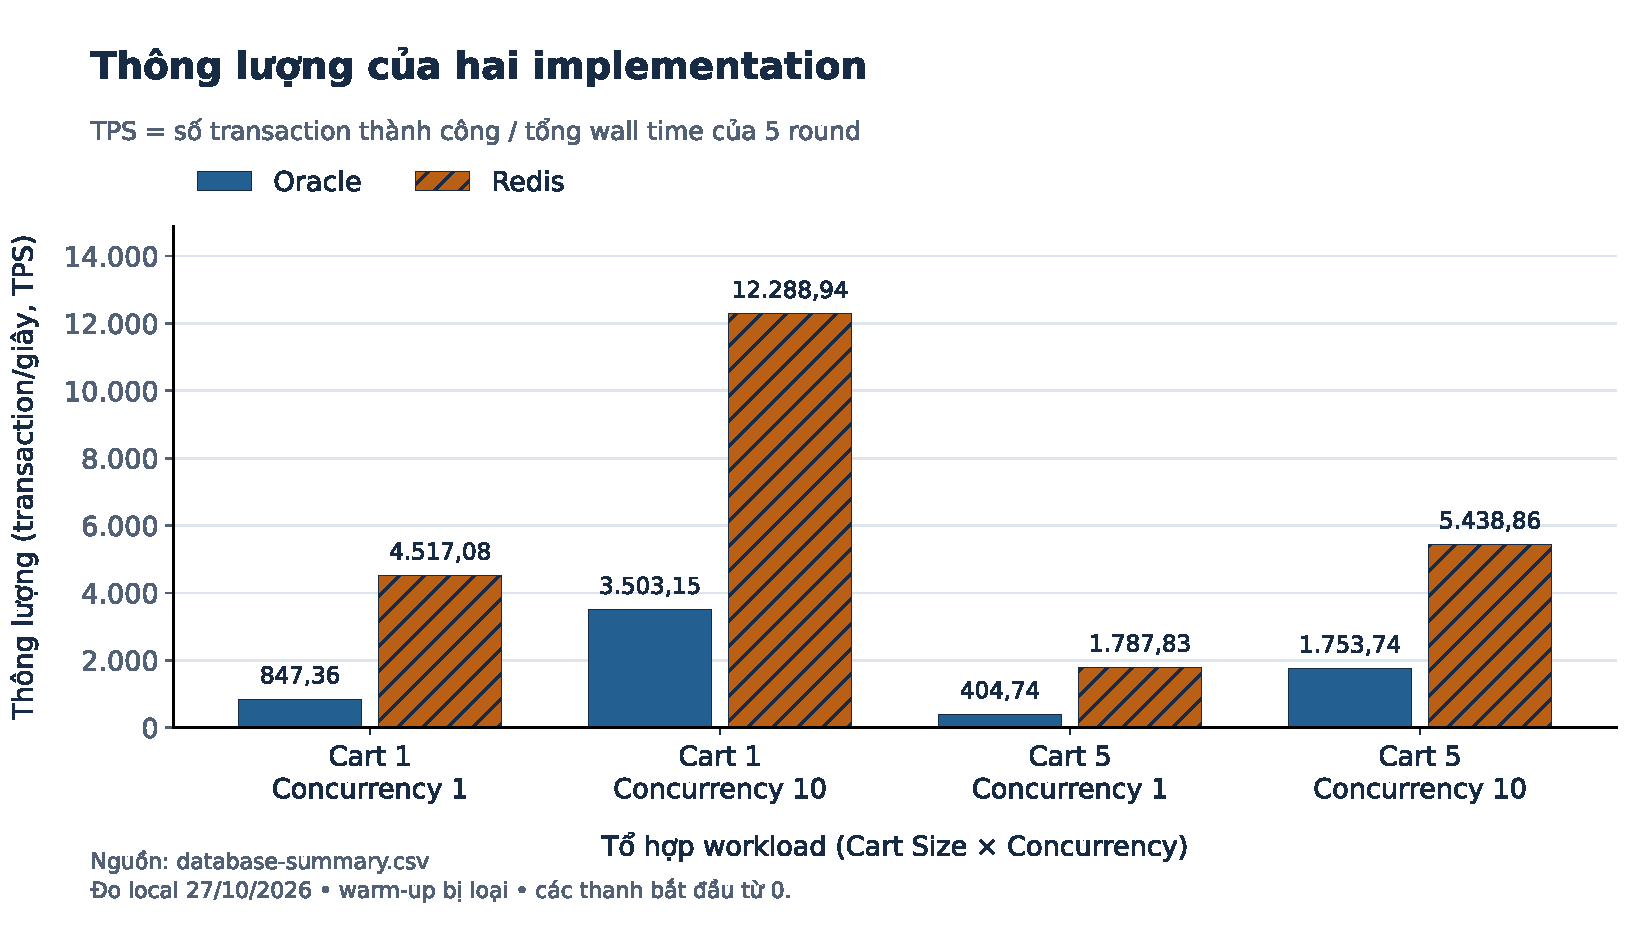
\includegraphics[width=\linewidth]{Pictures/Task_4/4.3-02-database-tps.pdf}
\caption[So sánh TPS Oracle–Redis theo bốn tổ hợp tải]{So sánh TPS Oracle–Redis theo bốn tổ hợp tải; dữ liệu từ bảng Database-level Benchmark.}\label{fig:tx-2}
\end{figure}
\textbf{Nhận xét kết quả.} Khi tăng Cart Size từ 1 lên 5, \textbf{p95 tăng và TPS giảm} ở cả hai implementation do một transaction phải xử lý nhiều dòng sản phẩm hơn. Khi tăng Concurrency từ 1 lên 10, \textbf{TPS tăng nhưng p95 cũng tăng}, phản ánh sự đánh đổi giữa thông lượng và thời gian xử lý từng giao dịch.

Redis có \textbf{p95 thấp hơn và TPS cao hơn trong cả bốn tổ hợp}. Ở Cart Size 5, Concurrency 10, Oracle đạt \textbf{6,1164 ms và 1.753,74 TPS}, trong khi Redis đạt \textbf{1,4019 ms và 5.438,86 TPS}. Kết quả này ghi nhận ưu thế của implementation Redis trong workload đã đo, nhưng chưa đủ để khẳng định Redis nhanh hơn Oracle đối với mọi transaction.

\begin{table}[!htbp]
\centering
\caption{Trung bình và độ lệch chuẩn của p95 qua năm round. Nguồn: \texttt{results/\allowbreak{}summary-\allowbreak{}20261027/\allowbreak{}database-\allowbreak{}summary.\allowbreak{}csv}.}\label{tab:tx-20}
\reporttablesetup
\begin{tabularx}{\linewidth}{|>{\hsize=0.65\hsize\linewidth=\hsize}L|>{\hsize=0.85\hsize\linewidth=\hsize}L|>{\hsize=1.25\hsize\linewidth=\hsize}L|>{\hsize=1.25\hsize\linewidth=\hsize}L|}
\hline
\rowcolor{ReportTableHead}
\reportheader{Cart Size} & \reportheader{Concurrency} & \reportheader{Oracle p95 TB \(\pm\) SD (ms)} & \reportheader{Redis p95 TB \(\pm\) SD (ms)} \\ \hline
1 & 1 & 1,2784 \(\pm\) 0,2425 & 0,1869 \(\pm\) 0,0451 \\ \hline
1 & 10 & 3,0004 \(\pm\) 0,1745 & 0,7042 \(\pm\) 0,0370 \\ \hline
5 & 1 & 2,6187 \(\pm\) 0,0733 & 0,4494 \(\pm\) 0,0388 \\ \hline
5 & 10 & 5,7613 \(\pm\) 0,5800 & 1,3381 \(\pm\) 0,2104 \\ \hline
\end{tabularx}
\end{table}
Chênh lệch giữa các round không đảo ngược xu hướng hiệu năng trên. Toàn bộ \textbf{8.000/8.000 transaction thành công}, không phát hiện invariant violation trong phạm vi hậu kiểm. Tuy nhiên, fixture chủ yếu độc lập giữa các worker, nên benchmark \textbf{chưa đo mức tranh chấp cao trên cùng sản phẩm}; khác biệt về schema, kết nối và durability cũng cần được xét khi diễn giải kết quả.

\txsubsection{Kết quả Application-level Benchmark}\label{sec:tx-3-3}
Phép đo HTTP sử dụng \textbf{k6 \(\rightarrow\) Vite proxy \(\rightarrow\) Spring Boot \(\rightarrow\) Oracle}, nhằm quan sát hiệu năng nghiệp vụ thực tế, \textbf{không so sánh Oracle với Redis ở tầng ứng dụng}. Một flow gồm đọc Cart, thêm 1 hoặc 5 sản phẩm, xem Checkout Preview, tạo Order, truy vấn danh sách/chi tiết Order và hủy Order. Do đó, \textbf{4.000 flow} tương ứng \textbf{36.000 HTTP request nghiệp vụ} (7 request/flow với Cart Size 1; 11 request/flow với Cart Size 5), không tính warm-up và login.

Bảng kết quả phân biệt \textbf{Checkout API} — riêng request tạo Order — với \textbf{Full Flow} — toàn bộ chuỗi thao tác nói trên.

\begin{table}[!htbp]
\centering
\caption{Kết quả Application-level Benchmark. Latency lấy từ các mẫu thành công; Flow/s tính theo số flow thành công trên tổng thời gian thực của năm round. Nguồn: \texttt{results/\allowbreak{}summary-\allowbreak{}20261027/\allowbreak{}http-\allowbreak{}summary.\allowbreak{}csv}.}\label{tab:tx-21}
\reporttablesetup
\scriptsize
\begin{tabularx}{\linewidth}{|>{\hsize=0.6\hsize\linewidth=\hsize}L|>{\hsize=1.05\hsize\linewidth=\hsize}L|>{\hsize=1.1\hsize\linewidth=\hsize}L|>{\hsize=1.1\hsize\linewidth=\hsize}L|>{\hsize=1.1\hsize\linewidth=\hsize}L|>{\hsize=1.1\hsize\linewidth=\hsize}L|>{\hsize=0.95\hsize\linewidth=\hsize}L|}
\hline
\rowcolor{ReportTableHead}
\reportheader{Cart Size} & \reportheader{Concurrency} & \reportheader{Checkout p50 (ms)} & \reportheader{Checkout p95 (ms)} & \reportheader{Full Flow p50 (ms)} & \reportheader{Full Flow p95 (ms)} & \reportheader{Flow/s} \\ \hline
1 & 1 & 2,9084 & 4,0406 & 14 & 18 & 68,34 \\ \hline
1 & 10 & 6,5273 & 8,9241 & 33 & 42 & 296,08 \\ \hline
5 & 1 & 4,9161 & 10,2897 & 30 & 62 & 27,73 \\ \hline
5 & 10 & 11,1444 & 14,7888 & 61 & 74 & 157,57 \\ \hline
\end{tabularx}
\end{table}
\begin{figure}[!htbp]
\centering
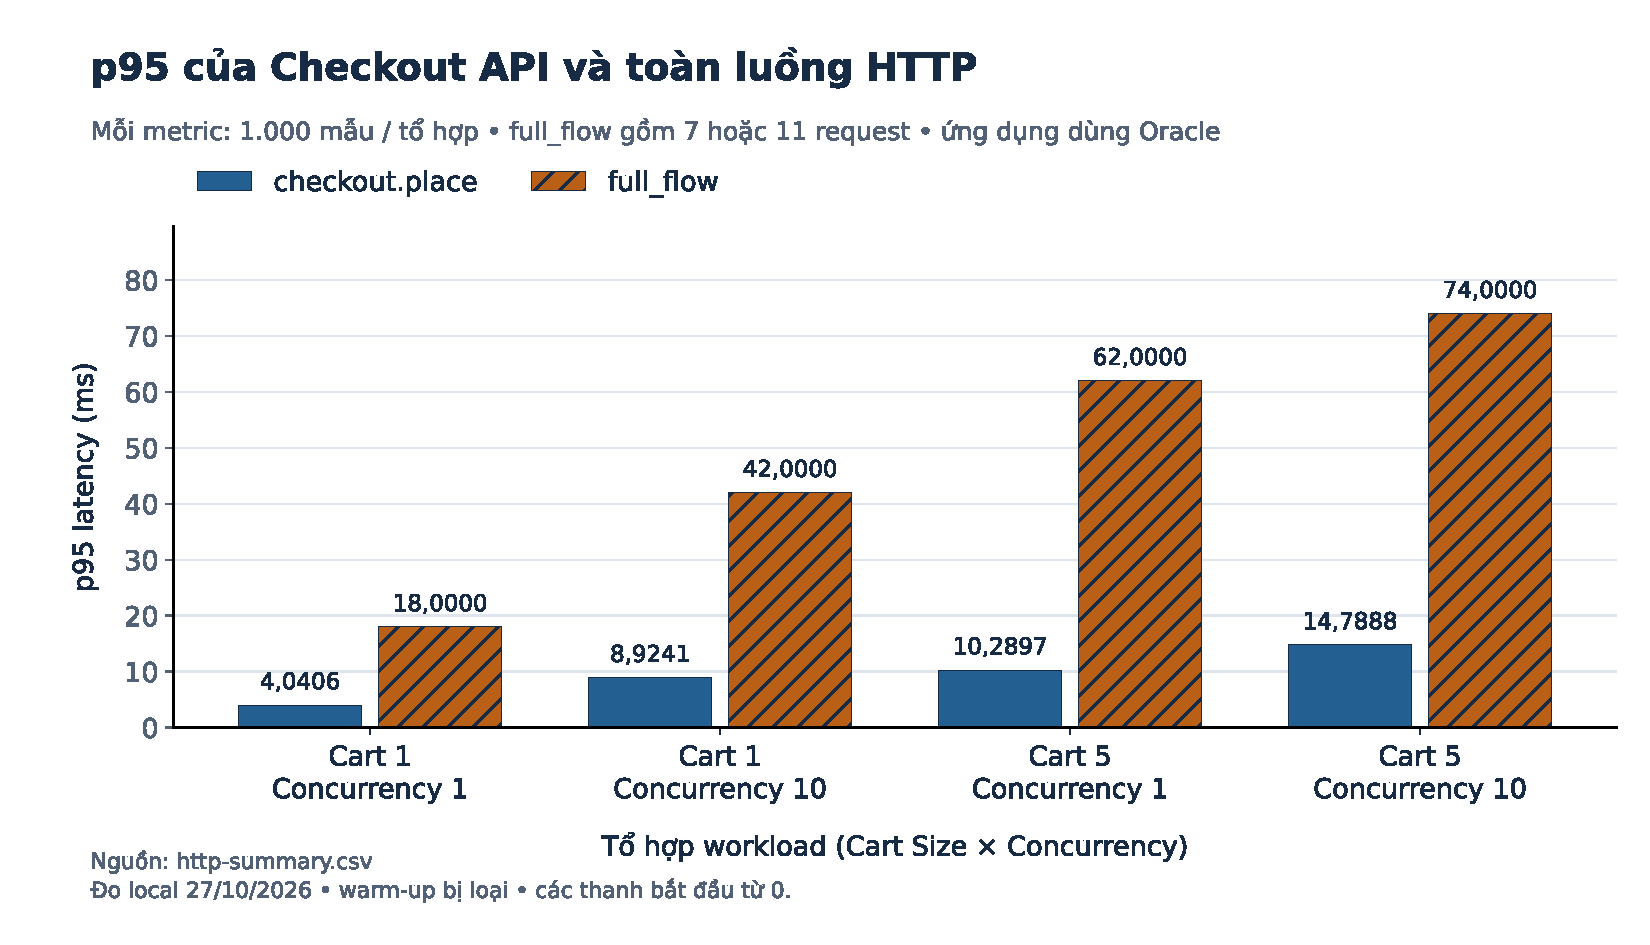
\includegraphics[width=\linewidth]{Pictures/Task_4/4.3-03-http-p95.pdf}
\caption[So sánh p95 Checkout API và Full Flow theo Cart Size/\allowbreak{}Concurrency]{So sánh p95 Checkout API và Full Flow theo Cart Size/\allowbreak{}Concurrency; dữ liệu từ bảng HTTP benchmark, đơn vị ms.}\label{fig:tx-3}
\end{figure}
\textbf{Nhận xét kết quả.} Khi Cart Size tăng từ 1 lên 5 ở Concurrency 1, Checkout p95 tăng từ \textbf{4,0406 lên 10,2897 ms}, Full Flow p95 tăng từ \textbf{18 lên 62 ms}. Nguyên nhân là Checkout phải xử lý nhiều sản phẩm và flow có thêm các request thêm Cart Item. Khi Concurrency tăng từ 1 lên 10, throughput tăng ở cả hai Cart Size (tương ứng \textbf{68,34 \(\rightarrow\) 296,08} và \textbf{27,73 \(\rightarrow\) 157,57 flow/s}), nhưng latency cũng tăng.

\textbf{Full Flow p95 cao hơn Checkout p95} vì chứa nhiều bước nghiệp vụ; không thể lấy chênh lệch hai phân vị làm chi phí chính xác của những API còn lại. Cả \textbf{4.000/4.000 flow hoàn tất}, không phát hiện invariant violation theo hậu kiểm. Kết quả cho thấy backend Oracle vận hành được dưới các mức tải đã thử, nhưng môi trường local và việc chưa tạo tranh chấp mạnh không đủ để suy ra hiệu năng production. \textbf{TPS database và Flow/s HTTP không thể so sánh trực tiếp} do khác đơn vị công việc.

\txsubsection{Đối chiếu tổng hợp và lựa chọn DBMS phù hợp}\label{sec:tx-3-4}
Từ các thí nghiệm về ACID và kết quả benchmark, có thể nhận thấy Oracle và Redis đều cung cấp những cơ chế hỗ trợ xử lý transaction, nhưng khác nhau đáng kể về phạm vi bảo đảm, cách kiểm soát lỗi và hiệu năng của các cách triển khai được khảo sát.

Bảng~\ref{tab:tx-22} tổng hợp những khác biệt có ảnh hưởng trực tiếp đến việc lựa chọn DBMS.

\begin{table}[!htbp]
\centering
\caption{Tổng hợp kết quả nghiên cứu Transaction trên Oracle và Redis.}\label{tab:tx-22}
\reporttablesetup
\begin{tabularx}{\linewidth}{|>{\hsize=0.65\hsize\linewidth=\hsize}L|>{\hsize=1.175\hsize\linewidth=\hsize}L|>{\hsize=1.175\hsize\linewidth=\hsize}L|}
\hline
\rowcolor{ReportTableHead}
\reportheader{Tiêu chí} & \reportheader{Oracle} & \reportheader{Redis} \\ \hline
\textbf{Atomicity} & Hỗ trợ COMMIT, ROLLBACK và SAVEPOINT; cho phép hoàn tác các thay đổi chưa commit trên nhiều bảng (A1, A3, D1). & MULTI/EXEC và Lua thực thi không bị command khác chen ngang, nhưng không tự hoàn tác những ghi thành công trước lỗi runtime (A4, A5). \\ \hline
\textbf{Consistency} & DBMS trực tiếp thực thi các constraint như PK, FK, UNIQUE và CHECK (C1, A2). & Các ràng buộc nghiệp vụ giữa những key phải được kiểm tra và bảo vệ trong đường ghi, chẳng hạn Lua guarded Checkout (C2). \\ \hline
\textbf{Isolation và Concurrency} & READ COMMITTED, row lock và SELECT FOR UPDATE hỗ trợ kiểm soát truy cập đồng thời; có cơ chế phát hiện deadlock (B1–B3). & Atomic command, WATCH và Lua hỗ trợ xử lý xung đột; cần lựa chọn cơ chế phù hợp với từng thao tác (B4, B5). \\ \hline
\textbf{Durability} & Sử dụng Redo Log và cơ chế phục hồi transaction. & Hỗ trợ RDB/AOF; môi trường khảo sát sử dụng AOF \texttt{everysec}. Chưa thực hiện crash-recovery benchmark để so sánh trực tiếp. \\ \hline
\textbf{Hiệu năng} & Có latency cao hơn và TPS thấp hơn trong workload database đã đo. & Có latency thấp hơn và TPS cao hơn trong cùng các tổ hợp khảo sát, nhưng hai implementation chưa tương đương hoàn toàn về ràng buộc và chi phí thực thi. \\ \hline
\end{tabularx}
\end{table}
\paragraph*{Đánh giá và quyết định đối với Oracle}

Trong bối cảnh thương mại điện tử, các nghiệp vụ Checkout, tạo đơn hàng và quản lý tồn kho đòi hỏi nhiều thao tác dữ liệu có quan hệ chặt chẽ. Oracle được đánh giá phù hợp với các yêu cầu này dựa trên ba cơ sở:

\begin{enumerate}[leftmargin=*,itemsep=2pt,topsep=4pt]
\item
\textbf{Khả năng quản lý transaction nhiều bước:} Hỗ trợ thực hiện và hoàn tác nhiều thay đổi trên các bảng trong cùng transaction, được kiểm chứng qua D1.

\item
\textbf{Bảo vệ tính toàn vẹn dữ liệu:} Các constraint được thực thi tại DBMS, giúp bảo vệ dữ liệu trên nhiều đường ghi khác nhau (A2, C1).

\item
\textbf{Kiểm soát truy cập đồng thời:} Row-level locking và SELECT FOR UPDATE hỗ trợ bảo vệ thao tác đọc–quyết định–ghi trong những nghiệp vụ có tranh chấp (B1–B3).

\end{enumerate}
\textbf{Quyết định:} Nhóm lựa chọn \textbf{Oracle làm nguồn dữ liệu chính (source of truth)} cho ShopFlash. Các nghiệp vụ Normal Checkout và Order Cancellation được thiết kế thực hiện trong Oracle transaction để bảo đảm việc tạo/cập nhật Order, Order Items, Inventory và Cart được xác nhận hoặc hoàn tác nhất quán. Dữ liệu giao dịch và kết quả mua Flash Sale thành công cũng được lưu trữ chính thức tại Oracle.

\paragraph*{Đánh giá và quyết định đối với Redis}

Redis thể hiện ưu thế về thời gian xử lý trong benchmark và cung cấp những cơ chế phù hợp với các thao tác có phạm vi dữ liệu hẹp, yêu cầu xử lý đồng thời cao:

\begin{enumerate}[leftmargin=*,itemsep=2pt,topsep=4pt]
\item
\textbf{Atomic Command:} Các thao tác như HINCRBY cho phép cập nhật bộ đếm nguyên tử mà không cần triển khai khóa riêng cho từng phép tăng/giảm (B4).

\item
\textbf{WATCH và Lua:} Hỗ trợ phát hiện xung đột hoặc kết hợp kiểm tra và cập nhật nhiều key trong một lần thực thi, phù hợp với việc kiểm soát quota (B4, B5).

\item
\textbf{Giới hạn transaction:} Không có full rollback tương đương Oracle khi phát sinh lỗi runtime sau ghi, nên cần validation trước ghi và cơ chế xử lý lỗi phù hợp (A5, C2).

\end{enumerate}
\textbf{Quyết định:} Nhóm lựa chọn \textbf{Redis cho Flash Sale runtime}, bao gồm kiểm soát quota, giới hạn mua theo người dùng và reservation tạm thời bằng Lua. Ngoài ra, Redis được sử dụng cho các dữ liệu dẫn xuất phục vụ tìm kiếm và thống kê, không thay thế Oracle làm nguồn dữ liệu giao dịch chính.

\paragraph*{Kết luận lựa chọn}

ShopFlash được thiết kế theo hướng kết hợp hai DBMS: \textbf{Oracle bảo đảm tính đúng đắn của dữ liệu giao dịch chính, Redis hỗ trợ các thao tác runtime cần tốc độ cao}. Đây là lựa chọn phù hợp với yêu cầu nghiệp vụ và những cơ chế đã nghiên cứu.
